% !TeX program = xelatex
\documentclass[a4paper,10pt]{article}

% ============================================================================
% កញ្ចប់បណ្ណាល័យ (Packages) – តាមលំនាំស្តង់ដារ អនុវិទ្យាល័យព្រះក្រសាំង (ls_plan.tex)
% បរិបទ៖ ថ្នាក់រៀនគ្មានស្លាយ LCD – បង្រៀនដោយប្រើក្ដារខៀន និងសន្លឹកកិច្ចការសិស្សស-ខ្មៅជាគោល
% ============================================================================
\usepackage[a4paper, left=0.95cm, right=0.95cm, top=0.85cm, bottom=0.92cm, footskip=0.52cm]{geometry}
\usepackage{amsmath}
\usepackage{unicode-math}
\usepackage{fontspec}
\usepackage{array, longtable, multirow, colortbl}
\usepackage[table]{xcolor}
\usepackage{enumitem}
\usepackage{pifont}
\usepackage{fancyhdr}
\usepackage{tikz}
\usetikzlibrary{calc, arrows.meta, angles, quotes, decorations.markings, positioning, babel}

\makeatletter
\let\@expl@@@mark@update@singlecol@structures@@\relax
\makeatother

% ============================================================================
% ការកំណត់ពុម្ពអក្សរផ្លូវការ (Cross-Platform Fonts Configuration)
% ============================================================================
\providecommand{\NGSFindFonts}{%
  \IfFileExists{C:/Windows/Fonts/cambria.ttc}{%
    \def\NGSSysPath{C:/Windows/Fonts/}%
    \def\NGSUserPath{C:/Users/KIT/AppData/Local/Microsoft/Windows/Fonts/}%
  }{%
    \IfFileExists{./fonts/KhmerOSsiemreap.ttf}{\def\NGSSysPath{./fonts/}\def\NGSUserPath{./fonts/}}{%
    \IfFileExists{../fonts/KhmerOSsiemreap.ttf}{\def\NGSSysPath{../fonts/}\def\NGSUserPath{../fonts/}}{%
    \IfFileExists{../../fonts/KhmerOSsiemreap.ttf}{\def\NGSSysPath{../../fonts/}\def\NGSUserPath{../../fonts/}}{%
    \IfFileExists{../../../fonts/KhmerOSsiemreap.ttf}{\def\NGSSysPath{../../../fonts/}\def\NGSUserPath{../../../fonts/}}{%
    \IfFileExists{../../../../fonts/KhmerOSsiemreap.ttf}{\def\NGSSysPath{../../../../fonts/}\def\NGSUserPath{../../../../fonts/}}{%
    \IfFileExists{../../../../../fonts/KhmerOSsiemreap.ttf}{\def\NGSSysPath{../../../../../fonts/}\def\NGSUserPath{../../../../../fonts/}}{%
    \IfFileExists{../../../../../../fonts/KhmerOSsiemreap.ttf}{\def\NGSSysPath{../../../../../../fonts/}\def\NGSUserPath{../../../../../../fonts/}}{%
      \def\NGSSysPath{../../../../../../../fonts/}\def\NGSUserPath{../../../../../../../fonts/}%
    }}}}}}}%
  }%
}
\NGSFindFonts

\setmathfont[Path={\NGSSysPath}, FontIndex=1, Scale=1.02]{cambria.ttc}
\defaultfontfeatures{Ligatures=TeX}

\setmainfont[
  Path={\NGSUserPath},
  Extension=.ttf,
  Script=Khmer,
  BoldFont={KhmerOSsiemreap},
  BoldFeatures={FakeBold=1.8},
  ItalicFont={KhmerOSsiemreap},
  ItalicFeatures={FakeSlant=0.25},
  BoldItalicFont={KhmerOSsiemreap},
  BoldItalicFeatures={FakeBold=1.8, FakeSlant=0.25}
]{KhmerOSsiemreap}

\newfontfamily\muol[Path={\NGSUserPath}, Extension=.ttf, Script=Khmer]{KhmerOSmuollight}
\newfontfamily\TimesEn[Path={\NGSSysPath}, Extension=.ttf, BoldFont={timesbd}, ItalicFont={timesi}, BoldItalicFont={timesbi}]{times}
\newfontfamily\NagaBold[Path={\NGSUserPath}, Extension=.ttf]{AKbalthom Naga Bold}
\newfontfamily\CalibriFont[Path={\NGSSysPath}, Extension=.ttf]{calibri}
\newfontfamily\Tacteing[Path={\NGSUserPath}]{TACTENG.TTF}
\newfontfamily\CourierBullet[Path={\NGSSysPath}, Extension=.ttf]{cour}
\newcommand{\wcirc}{{\CourierBullet\fontsize{9.5pt}{11pt}\selectfont o}}

\XeTeXlinebreaklocale "km"
\XeTeXlinebreakskip = 0pt plus 1pt minus 0.1pt

\definecolor{stepgray}{HTML}{D9D9D9}
\definecolor{headgray}{HTML}{F2F2F2}
\definecolor{boxgray}{HTML}{D9D9D9}
\definecolor{darkred}{HTML}{C00000}
\definecolor{red5e}{HTML}{FF0000}

\pagestyle{fancy}
\fancyhf{}
\renewcommand{\headrulewidth}{0pt}
\fancyfoot[R]{\CalibriFont\fontsize{11pt}{13pt}\selectfont\thepage}

\setlength{\parindent}{0pt}
\setlength{\parskip}{0pt}
\setlength{\tabcolsep}{3.8pt}

\newcolumntype{L}[1]{>{\raggedright\arraybackslash}p{#1}}

\newcommand{\en}[1]{{\TimesEn #1}}
\newcommand{\enbf}[1]{{\TimesEn\textbf{#1}}}
\newcommand{\unit}[1]{\,\text{\en{#1}}}
\newcommand{\fiveE}[1]{{\NagaBold\fontsize{9.5pt}{13pt}\selectfont\textcolor{red5e}{#1}}}
\newcommand{\timenote}[1]{\textcolor{darkred}{\textit{#1}}}
\newcommand{\redsub}[1]{\textcolor{darkred}{#1}}
\newcommand{\graybox}[1]{\colorbox{boxgray}{\strut\hspace{2pt}#1\hspace{2pt}}}
\newcommand{\ditem}{\tikz[baseline=-0.5ex]\fill (0,0.42ex) -- (0.42ex,0) -- (0,-0.42ex) -- (-0.42ex,0) -- cycle;\hspace{0.3em}}
\newcommand{\cnum}[1]{{\fontsize{10.5pt}{12pt}\selectfont\ding{\numexpr171+#1\relax}}\hspace{0.2em}}
\newcommand{\cfig}[1]{\par\vspace{4pt}{\centering #1\par}\vspace{4pt}}
\newcommand{\stepheader}[1]{\multicolumn{3}{|c|}{\cellcolor{stepgray}\muol #1} \\* \noalign{\hrule height 0.4pt}}
\newcommand{\tri}[1]{\ensuremath{\triangle #1}}
\newcommand{\ang}[1]{\ensuremath{\angle #1}}
\newcommand{\cg}{\ensuremath{\cong}}
\newcommand{\khmflourish}{{\Tacteing\fontsize{36pt}{14pt}\selectfont\raisebox{-5pt}{3}}}

\tikzset{
  tk1/.style={postaction={decorate},decoration={markings,mark=at position 0.50 with {\draw[black, line width=0.85pt](0,-0.095)--(0,0.095);}}},
  tk2/.style={postaction={decorate},decoration={markings,
    mark=at position 0.45 with {\draw[black, line width=0.85pt](0,-0.095)--(0,0.095);},
    mark=at position 0.55 with {\draw[black, line width=0.85pt](0,-0.095)--(0,0.095);}}},
  par1/.style={postaction={decorate},decoration={markings,mark=at position 0.52 with {\draw[black, line width=0.85pt](-0.07,0.08)--(0.05,0)--(-0.07,-0.08);}}}
}

% ============================================================================
% ម៉ាក្រូរូបភាពធរណីមាត្រស-ខ្មៅ (Proportional 4.2–7.2 cm B&W TikZ Diagrams)
% ============================================================================

% ១. រំលឹកមេរៀនទាក់ទង៖ ចតុកោណព្នាយសមបាត និងចតុកោណព្នាយកែង (រូបទី១-២ ទំ.១៨១) + បាតមធ្យមត្រីកោណ
\newcommand{\figPrereqTRAP}{%
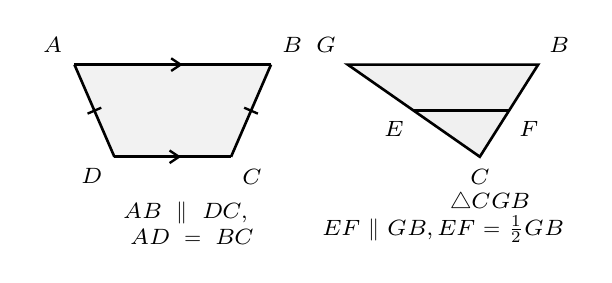
\begin{tikzpicture}[scale=0.78, every node/.style={font=\footnotesize, text=black}]
  % ឆ្វេង៖ ចតុកោណព្នាយសមបាត & កែង (ទំ.១៨១)
  \begin{scope}[shift={(0,0)}]
    \coordinate (D) at (0.65,0); \coordinate (C) at (2.55,0);
    \coordinate (A) at (0,1.50); \coordinate (B) at (3.20,1.50);
    \fill[gray!10] (A)--(B)--(C)--(D)--cycle;
    \draw[black, line width=0.95pt, par1] (A)--(B);
    \draw[black, line width=0.95pt, par1] (D)--(C);
    \draw[black, line width=0.95pt, tk1] (A)--(D);
    \draw[black, line width=0.95pt, tk1] (B)--(C);
    \node[above left=1pt] at (A) {$A$}; \node[above right=1pt] at (B) {$B$};
    \node[below right=1pt] at (C) {$C$}; \node[below left=1pt] at (D) {$D$};
    \node[anchor=north, text width=3.45cm, align=center] at (1.60,-0.42) {ចតុកោណព្នាយសមបាត៖\\បាត $AB\parallel DC$, ជ្រុង $AD=BC$};
  \end{scope}
  % ស្ដាំ៖ បាតមធ្យមត្រីកោណ EF = 1/2 GB
  \begin{scope}[shift={(4.45,0)}]
    \coordinate (G) at (0,1.50); \coordinate (B) at (3.10,1.50); \coordinate (C) at (2.15,0);
    \coordinate (E) at ($(G)!0.5!(C)$); \coordinate (F) at ($(B)!0.5!(C)$);
    \fill[gray!12] (G)--(B)--(C)--cycle;
    \draw[black, line width=0.95pt] (G)--(B)--(C)--cycle;
    \draw[black, line width=1.0pt] (E)--(F);
    \node[above left=1pt] at (G) {$G$}; \node[above right=1pt] at (B) {$B$}; \node[below=1pt] at (C) {$C$};
    \node[below left=0.5pt] at (E) {$E$}; \node[below right=0.5pt] at (F) {$F$};
    \node[anchor=north, text width=3.35cm, align=center] at (1.55,-0.42) {បាតមធ្យមត្រីកោណ $\tri{CGB}$៖\\$EF\parallel GB, EF=\frac{1}{2}GB$};
  \end{scope}
\end{tikzpicture}}

% ២. E1 Engage: កាំកណ្ដាលជណ្ដើរឈើរាងចតុកោណព្នាយ (AB=60cm, DC=36cm => EF=?)
\newcommand{\figEngageTRAP}{%
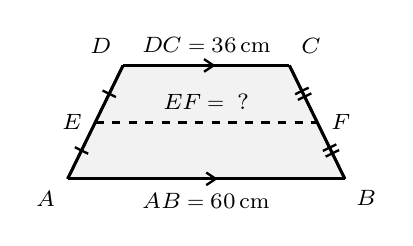
\begin{tikzpicture}[scale=0.80, every node/.style={font=\footnotesize, text=black}]
  \coordinate (A) at (0,0); \coordinate (B) at (4.40,0);
  \coordinate (D) at (0.88,1.80); \coordinate (C) at (3.52,1.80);
  \coordinate (E) at ($(A)!0.5!(D)$); \coordinate (F) at ($(B)!0.5!(C)$);
  \fill[gray!10] (A)--(B)--(C)--(D)--cycle;
  \draw[black, line width=1.1pt] (A)--(D) (B)--(C);
  \draw[black, line width=1.05pt, par1] (D)--(C);
  \draw[black, line width=1.05pt, par1] (A)--(B);
  \draw[black, line width=1.15pt, dashed] (E)--(F);
  \draw[black, line width=0.9pt, tk1] (A)--(E); \draw[black, line width=0.9pt, tk1] (E)--(D);
  \draw[black, line width=0.9pt, tk2] (B)--(F); \draw[black, line width=0.9pt, tk2] (F)--(C);
  \node[below left=1pt] at (A) {$A$}; \node[below right=1pt] at (B) {$B$};
  \node[above right=1pt] at (C) {$C$}; \node[above left=1pt] at (D) {$D$};
  \node[left=1.5pt] at (E) {$E$}; \node[right=1.5pt] at (F) {$F$};
  \node[above=1pt] at (2.20,1.80) {$DC = 36\unit{cm}$};
  \node[above=1pt] at (2.20,0.90) {$EF = \; ?$};
  \node[below=1.5pt] at (2.20,0) {$AB = 60\unit{cm}$};
\end{tikzpicture}}

% ៣. E2/E3: បន្ទាត់ជំនួយពីរបែប (ទំ.១៨២៖ DE || BC និង ទំ.១៨៣៖ បន្ទាត់ CE ប្រសព្វ BA ត្រង់ G)
\newcommand{\figAuxTRAP}{%
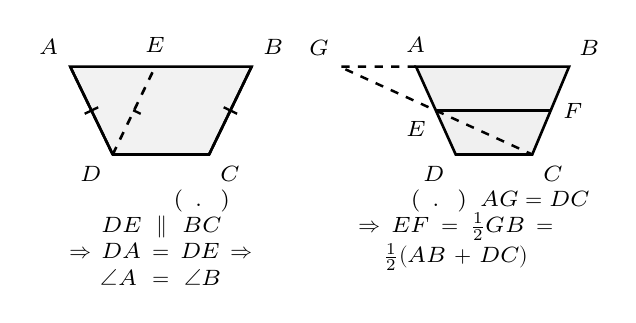
\begin{tikzpicture}[scale=0.72, every node/.style={font=\footnotesize, text=black}]
  % ឆ្វេង៖ ទ្រឹស្ដីបទទី១ (ទំ.១៨២៖ គូស DE || BC)
  \begin{scope}[shift={(0,0)}]
    \coordinate (D) at (0.75,0); \coordinate (C) at (2.45,0);
    \coordinate (A) at (0,1.55); \coordinate (B) at (3.20,1.55);
    \coordinate (E) at (1.50,1.55);
    \fill[gray!10] (A)--(B)--(C)--(D)--cycle;
    \draw[black, line width=0.95pt] (A)--(B)--(C)--(D)--cycle;
    \draw[black, line width=0.95pt, dashed, tk1] (D)--(E);
    \draw[black, line width=0.95pt, tk1] (A)--(D);
    \draw[black, line width=0.95pt, tk1] (B)--(C);
    \node[above left=1pt] at (A) {$A$}; \node[above=1.5pt] at (E) {$E$}; \node[above right=1pt] at (B) {$B$};
    \node[below left=1pt] at (D) {$D$}; \node[below right=1pt] at (C) {$C$};
    \node[anchor=north, text width=3.15cm, align=center] at (1.60,-0.45) {ទ្រឹស្ដីបទទី១ (ទំ.១៨២)៖ $DE\parallel BC$\\$\Rightarrow DA=DE \Rightarrow \ang{A}=\ang{B}$};
  \end{scope}
  % ស្ដាំ៖ ទ្រឹស្ដីបទទី៣ (ទំ.១៨៣៖ គូស CE កាត់បន្លាយ BA ត្រង់ G)
  \begin{scope}[shift={(4.75,0)}]
    \coordinate (G) at (0,1.55); \coordinate (A) at (1.35,1.55); \coordinate (B) at (4.05,1.55);
    \coordinate (D) at (2.05,0); \coordinate (C) at (3.40,0);
    \coordinate (E) at ($(A)!0.5!(D)$); \coordinate (F) at ($(B)!0.5!(C)$);
    \fill[gray!12] (A)--(B)--(C)--(D)--cycle;
    \draw[black, line width=0.95pt] (A)--(B)--(C)--(D)--cycle;
    \draw[black, line width=0.9pt, dashed] (A)--(G)--(E)--(C);
    \draw[black, line width=1.0pt] (E)--(F);
    \node[above left=0.5pt] at (G) {$G$}; \node[above=1.5pt] at (A) {$A$}; \node[above right=0.5pt] at (B) {$B$};
    \node[below left=1pt] at (D) {$D$}; \node[below right=1pt] at (C) {$C$};
    \node[below left=0.5pt] at (E) {$E$}; \node[right=1pt] at (F) {$F$};
    \node[anchor=north, text width=3.45cm, align=center] at (2.05,-0.45) {ទ្រឹស្ដីបទទី៣ (ទំ.១៨៣)៖ $AG=DC$\\$\Rightarrow EF=\frac{1}{2}GB=\frac{1}{2}(AB+DC)$};
  \end{scope}
\end{tikzpicture}}

% ៤. E4 Elaborate: គំរូទី១ (លំ.១០ក ទំ.១៨៦) & គំរូទី២ (លំហាត់គំរូ ទំ.១៨៤៖ O, H, G រត់ត្រង់គ្នា)
\newcommand{\figModelTRAP}{%
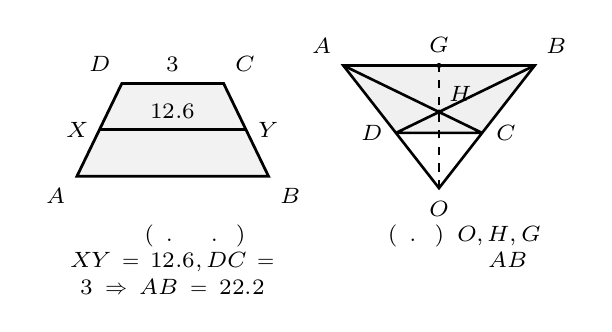
\begin{tikzpicture}[scale=0.76, every node/.style={font=\footnotesize, text=black}]
  % ឆ្វេង៖ លំហាត់ទី១០ក ទំ.១៨៦ (XY = 12.6, DC = 3 => AB = ?)
  \begin{scope}[shift={(0,0.20)}]
    \coordinate (D) at (0.75,1.55); \coordinate (C) at (2.45,1.55);
    \coordinate (A) at (0,0); \coordinate (B) at (3.20,0);
    \coordinate (X) at ($(A)!0.5!(D)$); \coordinate (Y) at ($(B)!0.5!(C)$);
    \fill[gray!10] (A)--(B)--(C)--(D)--cycle;
    \draw[black, line width=1.0pt] (A)--(B)--(C)--(D)--cycle;
    \draw[black, line width=1.0pt] (X)--(Y);
    \node[below left=1pt] at (A) {$A$}; \node[below right=1pt] at (B) {$B$};
    \node[above right=1pt] at (C) {$C$}; \node[above left=1pt] at (D) {$D$};
    \node[left=1pt] at (X) {$X$}; \node[right=1pt] at (Y) {$Y$};
    \node[above=0.5pt] at (1.60,1.55) {$3$}; \node[above=0.5pt] at (1.60,0.77) {$12.6$};
    \node[anchor=north, text width=3.45cm, align=center] at (1.60,-0.65) {គំរូទី១ (លំ.១០ក ទំ.១៨៦)៖\\$XY=12.6, DC=3 \Rightarrow AB=22.2$};
  \end{scope}
  % ស្ដាំ៖ លំហាត់គំរូ ទំ.១៨៤ (ចតុកោណព្នាយសមបាត ABCD => O, H, G រត់ត្រង់គ្នា)
  \begin{scope}[shift={(4.45,0)}]
    \coordinate (O) at (1.60,0);
    \coordinate (A) at (0,2.05); \coordinate (B) at (3.20,2.05);
    \coordinate (D) at ($(O)!0.45!(A)$); \coordinate (C) at ($(O)!0.45!(B)$);
    \coordinate (G) at (1.60,2.05);
    \coordinate (H) at (intersection of A--C and B--D);
    \fill[gray!12] (A)--(B)--(C)--(D)--cycle;
    \draw[black, line width=0.95pt] (O)--(A)--(B)--cycle;
    \draw[black, line width=0.95pt] (D)--(C) (A)--(C) (B)--(D);
    \draw[black, line width=0.9pt, dashed] (O)--(G);
    \fill[black] (G) circle (1.2pt) node[above=1pt] {$G$};
    \fill[black] (H) circle (1.2pt) node[above right=0.5pt] {$H$};
    \node[above left=1pt] at (A) {$A$}; \node[above right=1pt] at (B) {$B$};
    \node[left=1.5pt] at (D) {$D$}; \node[right=1.5pt] at (C) {$C$};
    \node[below=1pt] at (O) {$O$};
    \node[anchor=north, text width=3.45cm, align=center] at (1.60,-0.45) {គំរូទី២ (ទំ.១៨៤)៖ $O, H, G$\\ស្ថិតលើមេដ្យាទ័ររួមនៃ $AB$};
  \end{scope}
\end{tikzpicture}}

% ៥. E5 Evaluate: លំហាត់ទី១០ខ ទំ.១៨៦ + ទ្រឹស្ដីបទទី៤ (E, G, H, F រត់ត្រង់គ្នា)
\newcommand{\figPractTRAP}{%
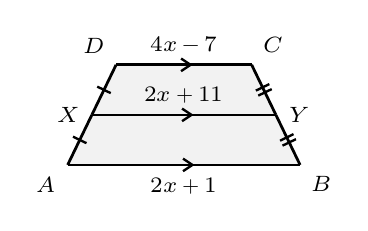
\begin{tikzpicture}[scale=0.82, every node/.style={font=\footnotesize, text=black}]
  \coordinate (A) at (0,0); \coordinate (B) at (3.60,0);
  \coordinate (D) at (0.75,1.55); \coordinate (C) at (2.85,1.55);
  \coordinate (X) at ($(A)!0.5!(D)$); \coordinate (Y) at ($(B)!0.5!(C)$);
  \fill[gray!10] (A)--(B)--(C)--(D)--cycle;
  \draw[black, line width=1.0pt, par1] (D)--(C);
  \draw[black, line width=1.0pt, par1] (A)--(B);
  \draw[black, line width=1.0pt, tk1] (A)--(X); \draw[black, line width=1.0pt, tk1] (X)--(D);
  \draw[black, line width=1.0pt, tk2] (B)--(Y); \draw[black, line width=1.0pt, tk2] (Y)--(C);
  \draw[black, line width=1.0pt, par1] (X)--(Y);
  \node[below left=1pt] at (A) {$A$}; \node[below right=1pt] at (B) {$B$};
  \node[above right=1pt] at (C) {$C$}; \node[above left=1pt] at (D) {$D$};
  \node[left=1.5pt] at (X) {$X$}; \node[right=1.5pt] at (Y) {$Y$};
  \node[above=1pt] at (1.80,1.55) {$4x-7$};
  \node[above=0.5pt] at (1.80,0.78) {$2x+11$};
  \node[below=1pt] at (1.80,0) {$2x+1$};
\end{tikzpicture}}

\begin{document}
\fontsize{10pt}{15.2pt}\selectfont

% -------------------- ក្បាលកិច្ចតែងការ (Header) --------------------
\begin{center}
  {\muol\fontsize{11pt}{16pt}\selectfont ព្រះរាជាណាចក្រកម្ពុជា}\\[2pt]
  {\muol\fontsize{10pt}{15pt}\selectfont ជាតិ សាសនា ព្រះមហាក្សត្រ}\\[1pt]
  \khmflourish
\end{center}

\vspace{-28pt}
{\muol\fontsize{9.5pt}{12.5pt}\selectfont
មន្ទីរអប់រំ យុវជន និងកីឡា ខេត្តកំពង់ធំ\\
ការិយាល័យអប់រំ យុវជន និងកីឡា ស្រុកកំពង់ស្វាយ\\
អនុវិទ្យាល័យព្រះក្រសាំង}

\vspace{1pt}
\begin{center}
  {\muol\fontsize{10pt}{14pt}\selectfont កិច្ចតែងការបង្រៀន}
\end{center}
\vspace{0pt}

% -------------------- ព័ត៌មានទូទៅ (Metadata) --------------------
{\renewcommand{\arraystretch}{0.95}
\hspace*{4.05cm}%
\begin{tabular}{@{}l l l@{}}
  - \hspace{0.35cm} មុខវិជ្ជា & : & គណិតវិទ្យា ថ្នាក់ទី៨ \\
  - \hspace{0.35cm} ចំណងជើងមេរៀន & : & មេរៀនទី១៣ ចតុកោណ \\
  - \hspace{0.35cm} ចំណងជើងរង & : & ២.៥ លក្ខណៈចតុកោណព្នាយ (ទំ.១៨១--១៨៤ និងទំ.១៨៦) \\
  - \hspace{0.35cm} រយៈពេល & : & ១ ម៉ោងសិក្សា (៥០ នាទី) \\
  - \hspace{0.35cm} បង្រៀនដោយ & : & ហុក ប៊ុនថែន \\
  - \hspace{0.35cm} កាលបរិច្ឆេទ & : & ថ្ងៃសុក្រ ៩កើត ខែមិគសិរ ព.ស.២៥៧០ (១៨ ធ្នូ ២០២៦) \\
\end{tabular}

\vspace{1pt}

% -------------------- I. វត្ថុបំណង --------------------
\textbf{I.} {\muol វត្ថុបំណង}\\[1pt]
\hspace*{0.55cm}%
\begin{tabular}{@{}l l L{14.2cm}@{}}
  \wcirc \hspace{0.25cm} វិជ្ជាសម្បទា & : & សិស្សពោលបានត្រឹមត្រូវនូវនិយមន័យចតុកោណព្នាយ ចតុកោណព្នាយសមបាត និងចតុកោណព្នាយកែង ព្រមទាំងទ្រឹស្ដីបទទាំង ៤៖ ទ្រឹស្ដីបទទី១--២ (មុំបាត និងអង្កត់ទ្រូងនៃចតុកោណព្នាយសមបាតប៉ុនគ្នា) ទ្រឹស្ដីបទទី៣ (បាតមធ្យម $EF\parallel AB\parallel DC$ និង $EF=\frac{1}{2}(AB+DC)$) និងទ្រឹស្ដីបទទី៤ (ចំណុចកណ្ដាលជ្រុងទ្រេត និងចំណុចកណ្ដាលអង្កត់ទ្រូងស្ថិតលើបន្ទាត់តែមួយ) តាមសៀវភៅគោល ទំ.១៨១--១៨៤ ។ \\
  \wcirc \hspace{0.25cm} បំណិនសម្បទា & : & សិស្សប្រើបន្ទាត់ជំនួយពីរបែប ($DE\parallel BC$ និងបន្ទាត់ $CE\cap BA=\{G\}$) ដើម្បីស្រាយបញ្ជាក់ទ្រឹស្ដីបទលើសន្លឹកកិច្ចការស-ខ្មៅ និងគណនារង្វាស់មុំ-ប្រវែងបាតមធ្យមដោយភ្ជាប់ហេតុផល \cnum{1}--\cnum{5} ។ \\
  \wcirc \hspace{0.25cm} ចរិយាសម្បទា & : & សិស្សមានទម្លាប់មិនច្រឡំរូបមន្តបាតមធ្យមចតុកោណព្នាយ $\frac{1}{2}(AB+DC)$ ទៅនឹងបាតមធ្យមត្រីកោណ $\frac{1}{2}AB$ ព្រមទាំងឃើញតម្លៃអនុវត្តក្នុងការធ្វើជណ្ដើរឈើ និងការរចនាសំណង់ ។ \\
\end{tabular}

\vspace{1pt}

% -------------------- II. សម្ភារៈឧបទេស --------------------
\textbf{II.} {\muol សម្ភារៈឧបទេស}\\[1pt]
\hspace*{0.55cm}$\bullet$ \hspace{0.35cm} សៀវភៅសិក្សាគោលគណិតវិទ្យាថ្នាក់ទី៨ (ទំ.១៨១--១៨៤ និងទំ.១៨៦) ក្ដារខៀន ដីស បន្ទាត់ក្រិត រ៉ាប់ព័រទ័រ និងសន្លឹកកិច្ចការសិស្សស-ខ្មៅ (\en{Worksheet\_TRAP1} ចំនួន ២ ទំព័រ \en{A4} ដោយគ្មានស្លាយ \en{LCD}) ។

\vspace{1pt}

% -------------------- III. វិធីសាស្រ្តបង្រៀន --------------------
\textbf{III.} {\muol វិធីសាស្រ្តបង្រៀន}\\[1pt]
\hspace*{0.45cm}%
\begin{tabular}{@{}l l L{14.85cm}@{}}
  $\bullet$ \hspace{0.25cm} គោលវិធី & : & សិស្សមជ្ឈមណ្ឌល (សិក្សាស៊ើបអង្កេតជាដៃគូលើសន្លឹកកិច្ចការបំពេញផ្ទាល់ គ្មានស្លាយ \en{LCD}) \\
  $\bullet$ \hspace{0.25cm} យុទ្ធវិធីបង្រៀន & : & គម្រូស្ថាបនានិយម \en{5Es} រួមបញ្ចូល \textbf{វិធីបំប្លែងរូបថ្មីទៅជារូបស្គាល់រួចតាមបន្ទាត់ជំនួយពីរបែប} (\en{Dual Auxiliary-Line Reduction — Stigler \& Hiebert, 1999; Palatnik \& Sigler, 2019}) \\
\end{tabular}
}

\vspace{1pt}

% -------------------- IV. ដំណើរការបង្រៀន --------------------
\textbf{IV.} {\muol ដំណើរការបង្រៀន}

\vspace{1pt}

\renewcommand{\arraystretch}{1.15}
\begin{longtable}{|L{5.50cm}|L{7.90cm}|L{4.80cm}|}
\hline
\rowcolor{headgray}
\multicolumn{1}{|c|}{\muol សកម្មភាពគ្រូ} &
\multicolumn{1}{c|}{\muol ខ្លឹមសារមេរៀន} &
\multicolumn{1}{c|}{\muol សកម្មភាពសិស្ស} \\
\hline
\endhead
\hline
\endfoot
\hline
\endlastfoot

% ==================== ជំហានទី១ (2min) ====================
\stepheader{ជំហានទី១ \enbf{(}រដ្ឋបាលថ្នាក់\enbf{)}}
$\bullet$ ពិនិត្យអវត្តមាន សណ្ដាប់ធ្នាប់ អនាម័យ និងសម្ភារៈធរណីមាត្រ (បន្ទាត់ក្រិត រ៉ាប់ព័រទ័រ)
&
$\bullet$ ពិនិត្យវត្តមាន និងសណ្ដាប់ធ្នាប់ថ្នាក់រៀន \par
$\bullet$ ត្រៀមបន្ទាត់ក្រិត និងរ៉ាប់ព័រទ័រសម្រាប់វាស់លើសន្លឹកកិច្ចការ
&
$\circ$ ប្រធានថ្នាក់រាយការណ៍អវត្តមាន និងត្រៀមឧបករណ៍ធរណីមាត្រ \\[3pt]

$\bullet$ រៀបចំសិស្សជាដៃគូពិភាក្សា រួចចែកសន្លឹកកិច្ចការ \en{Worksheet\_TRAP1} (២ ទំព័រ \en{A4}) ផ្កាប់លើតុ
&
$\bullet$ ការចាត់ដៃគូសិក្សា និងចែកសន្លឹកកិច្ចការស-ខ្មៅ
&
$\circ$ អង្គុយតាមដៃគូ និងទទួលសន្លឹកកិច្ចការទុកលើតុ \\
\hline

% ==================== ជំហានទី២ (9min: <=3 + 3 + E1 3) ====================
\stepheader{ជំហានទី២ \enbf{(}កិច្ចការផ្ទះ \enbf{+} ទំនាក់ទំនងមេរៀនថ្មី\enbf{)}}
\ditem \textbf{កំណែកិច្ចការផ្ទះ ($\le 3\unit{min}$)} \timenote{សង្ខេបខ្លីលើក្ដារខៀន}
&
{\centering\redsub{កំណែកិច្ចការផ្ទះ (ម៉ោងមុន៖ ការេ និងទ្រឹស្ដីបទចំណុចកណ្ដាល)}\par}
&
$\circ$ យកសៀវភៅកិច្ចការផ្ទះមកផ្ទៀងផ្ទាត់ \\[2pt]

$\bullet$ ផ្ទៀងផ្ទាត់ការសង់ការេ និងចម្លើយលំហាត់ទី២ យ៉ាងរហ័សលើក្ដារខៀន
&
$\bullet$ \textbf{លំ.១៖} គូស $AC=BD=6\unit{cm}$ កែងគ្នាត្រង់ចំណុចកណ្ដាល $O$ ($OA=OB=OC=OD=3\unit{cm}$) ។ \par
$\bullet$ \textbf{លំ.២៖} $E$ កណ្ដាល $AC \Rightarrow AC=10\unit{cm}$; $3x+2=\frac{1}{2}(16)=8 \Rightarrow x=2$ ។
&
$\circ$ ផ្ទៀងផ្ទាត់ចម្លើយ និងកែលម្អចំណុចខ្វះខាត \\[3pt]

\ditem \textbf{រំលឹកមេរៀនទាក់ទង ($3\unit{min}$)} \par
$\bullet$ គូសរូបលើក្ដារខៀន សួររំលឹក៖ ១. អ្វីទៅជាចតុកោណព្នាយ និងចតុកោណព្នាយសមបាត? ២. ក្នុង $\tri{CGB}$ បើ $E, F$ កណ្ដាល $CG, CB$ តើ $EF$ ស្មើប៉ុន្មាននៃ $GB$?
&
{\centering\redsub{រំលឹកមេរៀនទាក់ទងមេរៀនថ្មី}\par} \par
$\bullet$ \textbf{ចតុកោណព្នាយ} មានជ្រុងពីរស្របគ្នាហៅថា\textbf{បាត} ($AB\parallel DC$) និងជ្រុងពីរទៀតហៅថា\textbf{ជ្រុងទ្រេត}; បើជ្រុងទ្រេតស្មើគ្នា ($AD=BC$) ជា\textbf{ចតុកោណព្នាយសមបាត} ។ \par
$\bullet$ បាតមធ្យមត្រីកោណ៖ $EF\parallel GB$ និង $EF=\frac{1}{2}GB$ ។
&
$\circ$ ឆ្លើយផ្ទាល់មាត់អំពីបាត ជ្រុងទ្រេត និងបាតមធ្យមត្រីកោណ \\[3pt]

&
\cfig{\figPrereqTRAP}
& \\[3pt]

\fiveE{E1 - Engage (3min)} \timenote{(កុំទាន់ផ្ដល់ចម្លើយ)} \par
\ditem \textbf{បញ្ហាភ្ញាក់ផ្អើល «កាំកណ្ដាលនៃជណ្ដើរឈើរាងចតុកោណព្នាយ»៖} \par
$\bullet$ លើកស្ថានភាពជាងឈើធ្វើជណ្ដើរ $ABCD$ មានកាំក្រោម $AB=60\unit{cm}$ និងកាំលើ $DC=36\unit{cm}$ ចង់កាត់កាំកណ្ដាល $EF$!
&
{\centering\redsub{ស្ថានភាពបញ្ហា៖ កាំកណ្ដាលនៃជណ្ដើរឈើ}\par}
&
$\circ$ សង្កេតរូបជណ្ដើរឈើលើក្ដារខៀន និងលើសន្លឹកកិច្ចការផ្នែកទី១ \\[3pt]

&
\cfig{\figEngageTRAP}
& \\[3pt]

– \textbf{សំណួរបំផុស៖} «កូនជាង ក ថា $EF=\frac{1}{2}(60)=30\unit{cm}$ (យកតាមរូបមន្តត្រីកោណ)! តែមេជាង ខ ថា $EF=\frac{60+36}{2}=48\unit{cm}$! តើអ្នកណាត្រូវ? ហេតុអ្វីបានជាត្រូវបូកបាតទាំងពីរចែកនឹង ២?»
&
\textbf{ចម្ងល់គោលប្រចាំម៉ោង៖} \par
(១) តើចតុកោណព្នាយសមបាតមានលក្ខណៈមុំបាត និងអង្កត់ទ្រូងដូចម្ដេច? \par
(២) តើសង់បន្ទាត់ជំនួយបែបណា ដើម្បីបំប្លែងចតុកោណព្នាយទៅជាប្រលេឡូក្រាម និងត្រីកោណដែលយើងស្គាល់រួច?
&
$\circ$ ពិភាក្សាជាដៃគូ ៣០ វិនាទី រួចគូសធីកការទស្សន៍ទាយដំបូងក្នុងប្រអប់ \en{E1} លើសន្លឹកកិច្ចការ \\
\hline

% ==================== ជំហានទី៣ (17min: E2 11m + E3 6m) ====================
\stepheader{ជំហានទី៣ \enbf{(}ខ្លឹមសារមេរៀនថ្មី\enbf{)}}
\fiveE{E2 - Explore (11min)} \par
$\bullet$ សរសេរចំណងជើងរងលើក្ដារខៀន និងឱ្យសិស្សបើកសន្លឹកកិច្ចការទំព័រទី១ ផ្នែកទី២
&
២.៥ លក្ខណៈចតុកោណព្នាយ (ទំ.១៨១--១៨៤)
&
$\circ$ កត់ចំណងជើងរងចូលសៀវភៅសរសេរ និងបើកសន្លឹកកិច្ចការទំព័រទី១ \\[3pt]

\ditem \textbf{សកម្មភាពទី១៖ វាស់ផ្ទៀងផ្ទាត់ខ្នាតពិត 1:1 លើសន្លឹកកិច្ចការ ($4\unit{min}$)} \par
$\bullet$ ឱ្យដៃគូសិស្សវាស់ចតុកោណព្នាយសមបាតខ្នាតពិត ($AB=4.6\unit{cm}, DC=2.2\unit{cm}, AD=BC=2.0\unit{cm}$)៖ វាស់មុំបាត $\ang{A}, \ang{B}$, អង្កត់ទ្រូង $AC, BD$ និងបាតមធ្យម $EF$!
&
{\centering\textbf{លទ្ធផលពិសោធន៍វាស់ខ្នាតពិត 1:1}\par} \par
$\bullet$ មុំបាតប៉ុនគ្នា ($\ang{A}=\ang{B}\approx 53^\circ$) និងអង្កត់ទ្រូងប៉ុនគ្នា ($AC=BD\approx 3.8\unit{cm}$)! \par
$\bullet$ បាតមធ្យម៖ $EF = 3.4\unit{cm} = \frac{4.6+2.2}{2} =$ \graybox{$\frac{1}{2}(AB+DC)$}!
&
$\circ$ វាស់មុំបាត អង្កត់ទ្រូង និងបាតមធ្យមជាក់ស្ដែងលើសន្លឹកកិច្ចការ \\[3pt]

\ditem \textbf{សកម្មភាពទី២៖ បន្ទាត់ជំនួយពីរបែបស្រាយបញ្ជាក់ទ្រឹស្ដីបទទី១--៣ ($7\unit{min}$)} \par
$\bullet$ ដឹកនាំសិស្សបំពេញ \textbf{ផ្នែក ក (ទ្រឹស្ដីបទទី១--២ ទំ.១៨២)} ដោយគូសបន្ទាត់ជំនួយទី១៖ តាម $D$ គូស $DE\parallel BC$ កាត់ $AB$ ត្រង់ $E$
&
\textbf{ការបំប្លែងតាមបន្ទាត់ជំនួយពីរបែប៖} \par
$\bullet$ \textbf{ផ្នែក ក (ទ្រឹស្ដីបទទី១--២)៖} គូស $DE\parallel BC \Rightarrow EBCD$ ជាប្រលេឡូក្រាម $\Rightarrow DE=CB=DA \Rightarrow \tri{ADE}$ សមបាត $\Rightarrow \ang{A}=\ang{AED}=\ang{B}$! រួច $\tri{ADC}\cg\tri{DBC}$ (\textbf{ជ-ម-ជ}: $DA=CB, \ang{D}=\ang{C}, DC$ រួម) $\Rightarrow AC=DB$!
&
$\circ$ គូសបន្ទាត់ជំនួយ $DE\parallel BC$ និងបំពេញសម្រាយបញ្ជាក់ \textbf{ផ្នែក ក} \\[2pt]

$\bullet$ ដឹកនាំសិស្សបំពេញ \textbf{ផ្នែក ខ (ទ្រឹស្ដីបទទី៣ ទំ.១៨៣)} ដោយគូសបន្ទាត់ជំនួយទី២៖ គូស $CE$ កាត់បន្លាយបាត $BA$ ត្រង់ $G$
&
$\bullet$ \textbf{ផ្នែក ខ (ទ្រឹស្ដីបទទី៣ — បាតមធ្យម)៖} គូស $CE\cap BA=\{G\} \Rightarrow \tri{AGE}\cg\tri{EDC}$ (\textbf{ម-ជ-ម}) $\Rightarrow AG=DC$ និង $GE=EC$ ។ ក្នុង $\tri{CGB}$ អង្កត់ $EF$ ជាបាតមធ្យម $\Rightarrow DC\parallel EF\parallel AB$ និង $EF=\frac{1}{2}GB=\frac{1}{2}(AB+DC)$!
&
$\circ$ បំពេញសម្រាយបញ្ជាក់ \textbf{ផ្នែក ខ} រហូតទាញបានរូបមន្ត $EF=\frac{1}{2}(AB+DC)$ \\[3pt]

\fiveE{E3 - Explain (6min)} \par
\ditem \textbf{បង្គុំទ្រឹស្ដីបទទី១--៤ និងធនាគារហេតុផល \cnum{1}--\cnum{5}៖} \par
$\bullet$ ហៅតំណាងដៃគូឡើងបកស្រាយ រួចគ្រូសង្ខេបធនាគារហេតុផលផ្លូវការ (ទំ.១៨១--១៨៤)
&
\textbf{សង្ខេបធនាគារហេតុផល \cnum{1}--\cnum{5}៖} \par
\cnum{1} \textbf{និយមន័យ៖} ចតុកោណព្នាយមានបាតពីរស្របគ្នា ($AB\parallel DC$); បើជ្រុងទ្រេត $AD=BC$ ហៅថា\textbf{ចតុកោណព្នាយសមបាត}; បើមានមុំកែងមួយហៅថា\textbf{ចតុកោណព្នាយកែង} ។ \par
\cnum{2} \textbf{ទ្រឹស្ដីបទទី១៖} មុំបាតនៃចតុកោណព្នាយសមបាតប៉ុនគ្នា ($\ang{A}=\ang{B}, \ang{D}=\ang{C}$) ។
&
$\circ$ តំណាងដៃគូឡើងបកស្រាយ និងសិស្សបំពេញ \cnum{1}--\cnum{2} លើសន្លឹកកិច្ចការទំព័រទី២ \\[3pt]

&
\cfig{\figAuxTRAP}
& \\[3pt]

$\bullet$ សង្កត់ធ្ងន់លើទ្រឹស្ដីបទទី២ ទី៣ (បាតមធ្យម) និងទ្រឹស្ដីបទទី៤ (ចំណុចកណ្ដាលទាំង ៤ រត់ត្រង់គ្នា)
&
\cnum{3} \textbf{ទ្រឹស្ដីបទទី២៖} អង្កត់ទ្រូងនៃចតុកោណព្នាយសមបាតប៉ុនគ្នា ($AC=BD$) ។ \par
\cnum{4} \textbf{ទ្រឹស្ដីបទទី៣ (បាតមធ្យម)៖} $EF\parallel AB\parallel DC$ និង $EF=\frac{1}{2}(AB+DC)$ ។ \par
\cnum{5} \textbf{ទ្រឹស្ដីបទទី៤៖} ចំណុចកណ្ដាលជ្រុងទ្រេត $E, F$ និងចំណុចកណ្ដាលអង្កត់ទ្រូង $G, H$ ស្ថិតនៅលើបន្ទាត់តែមួយដែលស្របនឹងបាត ($GH=\frac{1}{2}|AB-DC|$) ។
&
$\circ$ កត់ត្រា \cnum{3}--\cnum{5} ចូលក្នុងប្រអប់ធនាគារហេតុផល \\
\hline

% ==================== ជំហានទី៤ (20min: E4 10m + E5 10m) ====================
\stepheader{ជំហានទី៤ \enbf{(}ពង្រឹង និងពង្រីកចំណេះដឹង\enbf{)}}
\fiveE{E4 - Elaborate (10min)} \par
\ditem \textbf{លំហាត់គំរូអនុវត្តចេញពីសៀវភៅគោល (លំ.១០ក ទំ.១៨៦ និង គំរូ ទំ.១៨៤)៖} \par
$\bullet$ ដឹកនាំសិស្សវិភាគគំរូទី១ (លំហាត់ទី១០ក ទំ.១៨៦៖ រកបាតធំពីបាតមធ្យម)
&
{\muol លំហាត់គំរូទី១} \textbf{(លំហាត់ទី១០ក ទំ.១៨៦)៖} \par
ក្នុងចតុកោណព្នាយ $ABCD$ ($AB\parallel DC$) មានបាតមធ្យម $XY=12.6$ និងបាតតូច $DC=3$ ។ គណនាប្រវែងបាតធំ $AB$ ។
&
$\circ$ អានប្រធានគំរូទី១ និងរៀបសមីការតាមរូបមន្ត \cnum{4} \\[2pt]

$\bullet$ ដឹកនាំសិស្សវិភាគគំរូទី២ (លំហាត់គំរូ ទំ.១៨៤៖ ចំណុច $O, H, G$ រត់ត្រង់គ្នា)
&
{\muol លំហាត់គំរូទី២} \textbf{(លំហាត់គំរូ ទំ.១៨៤)៖} \par
គេមានចតុកោណព្នាយសមបាត $ABCD$ ($AB\parallel DC$) ចំណុច $G$ កណ្ដាលនៃ $AB$, $O=AD\cap BC$ និង $H=AC\cap BD$ ។ បង្ហាញថា $O, H$ និង $G$ ស្ថិតនៅលើបន្ទាត់តែមួយ ។
&
$\circ$ សង្កេតរូបគំរូទី២ និងគូសឆ្នូតស្មើគ្នាលើត្រីកោណសមបាត $\tri{OAB}$ និង $\tri{HAB}$ \\[3pt]

&
\cfig{\figModelTRAP}
& \\[3pt]

$\bullet$ សួរបំផុសគំរូទី១ និងគំរូទី២៖ «តើមេដ្យាននៃត្រីកោណសមបាតដើរតួជាបន្ទាត់ពិសេសអ្វីនៃបាត $AB$?»
&
\textbf{ដំណោះស្រាយសង្ខេប៖} \par
$\bullet$ \textbf{គំរូទី១៖} តាម \cnum{4}: $\frac{AB+DC}{2}=XY \Rightarrow AB+3=2(12.6)=25.2 \Rightarrow$ \graybox{$AB=22.2$} ។
&
$\circ$ បំពេញចម្លើយគំរូទី១ លើសន្លឹកកិច្ចការ \\[2pt]

$\bullet$ ដឹកនាំសម្រាយបញ្ជាក់គំរូទី២ តាមបន្ទាត់មេដ្យាទ័ររួមនៃ $AB$ និងសួរឆ្លុះបញ្ចាំង \en{EIA}
&
$\bullet$ \textbf{គំរូទី២៖} $\ang{OAB}=\ang{OBA}\Rightarrow \tri{OAB}$ សមបាត $\Rightarrow$ មេដ្យាន $OG$ ជា\textbf{មេដ្យាទ័រ}នៃ $AB$ (១) ។ $\tri{ADC}\cg\tri{BDC}\Rightarrow \ang{DAC}=\ang{DBC}\Rightarrow \ang{CAB}=\ang{DBA}\Rightarrow \tri{HAB}$ សមបាត $\Rightarrow$ មេដ្យាន $HG$ ក៏ជា\textbf{មេដ្យាទ័រ}នៃ $AB$ (២) ។ តាម (១) និង (២) \graybox{$O, H, G$ ស្ថិតលើបន្ទាត់តែមួយ}! \par
$\bullet$ \textbf{គន្លឹះ \en{EIA}៖} អង្កត់ភ្ជាប់ចំណុចកណ្ដាលបាតទាំងពីរនៃចតុកោណព្នាយសមបាត ជាអ័ក្សឆ្លុះរបស់វា!
&
$\circ$ បំពេញជំហានគំរូទី២ និងកត់សម្គាល់អ័ក្សឆ្លុះនៃចតុកោណព្នាយសមបាត \\[3pt]

\fiveE{E5 - Evaluate (10min)} \par
\ditem \textbf{លំហាត់ប្រតិបត្តិចេញពីសៀវភៅគោល ($6.5\unit{min}$, លំហាត់ទី១០ខ ទំ.១៨៦)៖} \par
$\bullet$ ឱ្យសិស្សធ្វើលំហាត់ទី១០ខ ទំព័រ ១៨៦ លើសន្លឹកកិច្ចការដោយឯករាជ្យ ៤ នាទី
&
{\muol លំហាត់ប្រតិបត្តិ} \textbf{(លំហាត់ទី១០ខ សៀវភៅគោល ទំ.១៨៦)៖} \par
ក្នុងចតុកោណព្នាយ $ABCD$ ($AB\parallel DC$) មានបាតមធ្យម $XY=2x+11$, បាត $DC=4x-7$ និងបាត $AB=2x+1$ ។ គណនាតម្លៃ $x$ រួចទាញរកប្រវែង $XY$ ។
&
$\circ$ រៀបសមីការ $AB+DC=2\cdot XY$ និងដោះស្រាយរក $x$ ដោយឯករាជ្យ \\[3pt]

&
\cfig{\figPractTRAP}
& \\[3pt]

$\bullet$ ឱ្យដៃគូសិស្សប្ដូរផ្ទៀងផ្ទាត់ចម្លើយ (\en{Peer-Check}) ២.៥ នាទី និងឆ្លើយបិទបញ្ហាជណ្ដើរ \en{E1}
&
$\bullet$ \textbf{ចម្លើយប្រតិបត្តិ៖} តាម \cnum{4}: $(2x+1)+(4x-7)=2(2x+11) \Rightarrow 6x-6=4x+22 \Rightarrow 2x=28 \Rightarrow$ \graybox{$x=14$} ។ នាំឱ្យ $XY=2(14)+11=$ \graybox{$39$} ។ \par
$\bullet$ \textbf{បិទបញ្ហា E1៖} មេជាង ខ ត្រឹមត្រូវ! កាំកណ្ដាលជណ្ដើរជាបាតមធ្យមចតុកោណព្នាយ $EF=\frac{60+36}{2}=48\unit{cm}$!
&
$\circ$ ប្ដូរផ្ទៀងចម្លើយប្រតិបត្តិជាមួយដៃគូ និងសរសេរចម្លើយបិទបញ្ហា \en{E1} \\[3pt]

\ditem \textbf{សំណួរត្រួតពិនិត្យរហ័ស \en{Exit Check A--D} ($3.5\unit{min}$)៖} \par
$\bullet$ ឱ្យសិស្សគូសរង្វង់ចម្លើយត្រឹមត្រូវលើសន្លឹកកិច្ចការ រួចលើកម្រាមដៃ ១--៤ បង្ហាញចម្លើយ
&
\textbf{សំណួរ Exit Check (មុំចតុកោណព្នាយសមបាត និងបាតមធ្យម)៖} \par
«ក្នុងចតុកោណព្នាយសមបាត $ABCD$ ($AB\parallel DC$) បើបាត $AB=14\unit{cm}, DC=6\unit{cm}$ និងមុំ $\ang{A}=70^\circ$ តើបាតមធ្យម $EF$ និងមុំ $\ang{D}$ ស្មើប៉ុន្មាន?» \par
\en{A.} $10\unit{cm}$ និង $70^\circ$ \quad \en{B.} $7\unit{cm}$ និង $110^\circ$ \par
\en{C.} $20\unit{cm}$ និង $110^\circ$ \quad \graybox{\enbf{D.} $10\unit{cm}$ និង $110^\circ$ \ding{51}}
&
$\circ$ គូសរង្វង់ជ្រើសរើស \textbf{D} លើសន្លឹកកិច្ចការ និងលើកម្រាមដៃ ៤ ផ្ទៀងផ្ទាត់ជាមួយគ្រូ \\
\hline

% ==================== ជំហានទី៥ (<=2min) ====================
\stepheader{ជំហានទី៥ \enbf{(}កិច្ចការផ្ទះ \enbf{+} បណ្ដាំផ្ញើ\enbf{)}}
$\bullet$ កត់ត្រាកិច្ចការផ្ទះលើក្ដារខៀន (មានបោះពុម្ពស្រាប់នៅផ្នែកទី៦ នៃសន្លឹកកិច្ចការទំព័រទី២)
&
{\centering{\muol កិច្ចការផ្ទះ} \textbf{(លំហាត់ទី១១ ទំ.១៨៦ និងសំយោគទ្រឹស្ដីបទទី៤)}\par} \par
១. \textbf{លំហាត់ទី១១ (ទំ.១៨៦)៖} ក្នុងចតុកោណព្នាយសមបាត $ABCD$ ដែលមាន $BC\parallel AD$ និងមុំ $\ang{A}=67^\circ$ ចូរគណនារង្វាស់មុំ $\ang{B}, \ang{C}$ និង $\ang{D}$ ។ \par
២. \textbf{លំហាត់ទី២៖} ក្នុងចតុកោណព្នាយ $ABCD$ ($AB\parallel DC, AB=18\unit{cm}, DC=10\unit{cm}$) មាន $E, F$ កណ្ដាលជ្រុងទ្រេត $AD, BC$ និង $G, H$ កណ្ដាលអង្កត់ទ្រូង $AC, BD$ ។ គណនាប្រវែង $EF, EG, HF$ និង $GH$ ។
&
$\circ$ កត់ត្រាកិច្ចការផ្ទះ និងទុកដាក់សន្លឹកកិច្ចការក្នុងសៀវភៅសរសេរ \\[3pt]

$\bullet$ ណែនាំឱ្យអានមេរៀនទី១៤ ជាមុន និងផ្ដាំផ្ញើវិន័យសិក្សា
&
$\bullet$ \textbf{អានជាមុន៖} មេរៀនទី១៤ ផ្ទៃក្រឡាពហុកោណ — ១. ផ្ទៃក្រឡាប្រលេឡូក្រាម (ទំ.១៨៧--១៩០) \par
$\bullet$ \textbf{បណ្ដាំផ្ញើ៖} រំលឹកលក្ខណៈចតុកោណទាំងអស់នៃមេរៀនទី១៣ និងធ្វើកិច្ចការផ្ទះឱ្យទៀងទាត់ ។
&
$\circ$ ទទួលបណ្ដាំផ្ញើ និងជម្រាបលាគ្រូ \\

\end{longtable}

\vspace{6pt}

% -------------------- ហត្ថលេខា (Signature Block) --------------------
\begin{flushright}
\begin{minipage}{7.6cm}
\centering
ថ្ងៃសុក្រ ៩កើត ខែមិគសិរ ឆ្នាំមមី អដ្ឋស័ក ពុទ្ធសករាជ ២៥៧០\\[2pt]
កំពង់ស្វាយ, ថ្ងៃទី១៨ ខែធ្នូ ឆ្នាំ២០២៦\\[4pt]
{\muol គ្រូបង្រៀន}\\[32pt]
\hfill{\muol ហុក ប៊ុនថែន}\hspace*{1.0cm}
\end{minipage}
\end{flushright}

\end{document}
